\documentclass[12pt]{article}

\usepackage[utf8]{inputenc}
\usepackage{latexsym,amsfonts,amssymb,amsthm,amsmath}
\usepackage{tikz}
\usepackage{stanli}
\usetikzlibrary{shapes,calc,through,3d,patterns}
\usetikzlibrary{arrows.meta,decorations.pathreplacing,angles,quotes}
\usepackage{multicol}
\usepackage{geometry}
\usepackage{mathtools}
\usepackage{siunitx}
\usepackage{booktabs}

\setlength{\parindent}{0in}
\setlength{\oddsidemargin}{-0.25in}
\setlength{\textwidth}{7in}
\setlength{\textheight}{9.3in}
\setlength{\topmargin}{-1in}
\setlength{\headheight}{18pt}

\newcommand\blfootnote[1]{%
    \begingroup
    \renewcommand\thefootnote{}\footnote{#1}%
    \addtocounter{footnote}{-1}%
    \endgroup
}

\definecolor{darkred}{rgb}{0.6,0,0}

\newcommand{\bolddelta}{\boldsymbol\delta}
\newcommand{\boldxi}{\boldsymbol\xi}

\begin{document}

\noindent ME473 - Dynamic finite element analysis of structures\hfill EPFL\\
Stefano Burzio \hfill 2025\\
\vspace{0.3cm}

\hspace*{\fill}\textbf{\Large Problem set 5}\hspace*{\fill}

\hrulefill

\subsection*{Problem 1}
Consider the two-dimensional truss structure depicted in the figure below. The structure consists of two linear elastic truss elements, each characterized by a modulus of elasticity $E$ and a constant cross-sectional area $A$. The structure is modeled using three nodes and two finite elements within a global coordinate system whose origin is located at node 1.
\begin{center}
    \begin{tikzpicture}
        % Nodes
        \def\c{0.7071}
        \def\s{0.7071}
        \coordinate (1) at (0,0);
        \coordinate (2) at (2.5*\s,2.5*\c);
        \coordinate (3) at (0,5);
        %Supports 
        \point{a}{0}{5};
        \point{b}{2.5*\s}{2.5*\c};
        \support{1}{a}[-180];
        \support{1}{b}[-180];
        % Members
        \draw[ultra thick] (1) -- (2);
        \draw[ultra thick] (3) -- (1);
        \draw[thick] (1.3,0.7) circle(0.2cm);
        \node at (1.3,0.7) {1};
        \draw[thick] (-0.5,2.5) circle(0.2cm);
        \node at (-0.5,2.5) {2};
        % Force at 1
        \draw[thick,latex-] (0.1,0) -- ++(1.2,0) node[midway,below] {25 kN};
        % Points
        \node[below left=1pt,darkred] at (1) {1};
        \node[below right=1pt,darkred] at (2) {2};
        \node[below right=1pt,darkred] at (3) {3};
        % Angle
        \draw pic["45$^\circ$", draw=black, angle eccentricity=1.3, angle radius=1cm]{angle=2--1--3};
        % Dimensions
        \draw[|-|] ($(3)+(-0.8,0)$) -- node[left] {10 m} ($(1)+(-0.8,0)$);
        \draw[|-|] ($(1)+(-1,0)$) -- node[midway, left] {$5\cos(45^\circ)$} (-1,2.5*\s);
        % Axes
        \draw[-latex,  thin, darkred] (1) -- ++(2,0) node[right] {$x$};
        \draw[-latex,  thin, darkred] (1) -- ++(0,2) node[right] {$y$};
        % Pins
        \draw[thick,fill=white] (3) circle (3pt);
        \draw[thick,fill=white] (2) circle (3pt);
        \draw[thick,fill=white] (1) circle (3pt);
    \end{tikzpicture}
\end{center}

The truss is subjected to an external horizontal load of $25$ kN applied at node 1.
\begin{enumerate}
    \item[a)] Degree of freedom classification: using the finite element discretization, the system has a total of six degrees of freedom, two per node. Identify which of these degrees of freedom are constrained due to boundary conditions, and which are unconstrained.
    \item[b)] Reduced system formulation: by eliminating the constrained degrees of freedom, compute the reduced stiffness matrix and the reduced applied loads vector corresponding to the unconstrained degrees of freedom of the structure.
    \item[c)] Displacement calculation: solve the reduced system to obtain the displacements at the unconstrained degrees of freedom.
    \item[d)] Stress evaluation: using the computed displacements, determine the approximate axial stress in each truss element. Then, provide a physical interpretation of the results: which member is in tension or compression, and why?
\end{enumerate}

\newpage
\subsection*{Problem 2}
Consider the two-dimensional truss structure illustrated below, composed of three inclined bars made of structural steel. The material and geometric properties of each member are as follows:
\begin{itemize}
    \item Young’s modulus: $E = 210 \, \text{GPa}$
    \item Cross-sectional area: $A = 6.45 \times 10^{-4} \, \text{m}^2$
    \item Density $\rho = 7800 \, \text{kg/m}^3$
\end{itemize}

Node 1 is fully constrained, while node 3 is constrained in the vertical ($y$) direction only. These boundary conditions result in a system with three unconstrained degrees of freedom.
\begin{center}
    \begin{tikzpicture}[]
        % Nodes coordinates
        \coordinate (1) at (0,0);
        \coordinate (2) at (0,5);
        \coordinate (3) at (5,0);
        % Members (bars)
        \draw[ultra thick] (1) -- (2);
        \draw[ultra thick] (2) -- (3);
        \draw[ultra thick] (3) -- (1);
        \draw[thick] (-0.5,2.5) circle(0.2cm);
        \node at (-0.5,2.5) {1};
        \draw[thick] (2.5,-0.5) circle(0.2cm);
        \node at (3,3) {2};
        \draw[thick] (3,3) circle(0.2cm);
        \node at (2.5,-0.5) {3};
        \draw[thick] (2.5,-0.5) circle(0.2cm);
        % Force at 1
        \draw[thick,latex-] (-0.1,5) -- ++(-1.2,0) node[midway,above] {22 kN};
        % Points
        \node[above right=1pt,darkred] at (1) {1};
        \node[above right=1pt,darkred] at (2) {2};
        \node[above right=1pt,darkred] at (3) {3};
        %Supports 
        \point{a}{0}{0};
        \point{b}{5}{0};
        \support{1}{a};
        \support{2}{b};
        \draw [thick] (4.70,-0.55) circle [radius=0.05];
        \draw [thick] (5.00,-0.55) circle [radius=0.05];
        \draw [thick] (5.30,-0.55) circle [radius=0.05];
        %Length 
        \draw[|-|] (0,-1) -- node[below] {$6$ m} (5,-1);
        \draw[|-|] (-1,0) -- node[left] {$6$ m} (-1,5);
        % Pins
        \draw[thick,fill=white] (1) circle (3pt);
        \draw[thick,fill=white] (2) circle (3pt);
        \draw[thick,fill=white] (3) circle (3pt);
    \end{tikzpicture}
\end{center}
Develop a \texttt{MATLAB} script that performs the following tasks:
\begin{enumerate}
    \item Assemble the global stiffness matrix $\mathbf{K}$ and consistent mass matrix $\mathbf{M}$ of the truss structure.
    \item Compute the natural frequencies $\omega_i$ and the corresponding mode shapes $\boldsymbol{\phi}_i$.
    \item Determine the time response of the structure when subjected to a constant external force $f = 22 \, \text{kN}$ applied at node 1 along the horizontal ($x$) direction.
          \begin{itemize}
              \item[a)]Use modal decomposition to transform the coupled second-order differential system
                    \[
                        \mathbf{M} \ddot{\mathbf{q}}(t) + \mathbf{K} \mathbf{q}(t) = \mathbf{f}(t)
                    \]
                    into a system of uncoupled scalar equations by expressing the displacement vector as $\mathbf{q}(t) = \boldsymbol{\Phi} \, \mathbf{z}(t)$, where $\boldsymbol{\Phi}$ is the modal matrix formed by mass-normalized mode shapes.
              \item[b)]More precisely, apply the orthogonality conditions
                    \[
                        \boldsymbol{\Phi}^T \mathbf{M} \boldsymbol{\Phi} = \mathbf{I}, \qquad \boldsymbol{\Phi}^T \mathbf{K} \boldsymbol{\Phi} = \boldsymbol{\Lambda}
                    \]
                    with $\boldsymbol{\Lambda} = \text{diag}(\lambda_1, \dots, \lambda_n)$, to derive and solve the uncoupled system governing the modal coordinates $\mathbf{z}(t)$.
              \item[c)] Solve the uncoupled system and compute the time response vector $\mathbf{q}$ at the unconstrained degrees of freedom.
          \end{itemize}

\end{enumerate}


\end{document}